\documentclass[11pt]{article}

\usepackage{amssymb}
\usepackage{amsmath, esint}
\usepackage{amsthm}
\usepackage{array}
\usepackage{longtable}
\usepackage{mathtools}
\usepackage{pdfpages}
\usepackage{fancyhdr}
\usepackage[figurename=Figure]{caption}
\usepackage{empheq}
\usepackage{mdframed}
\usepackage[a4paper, left=1in,right=1in,top=1in,bottom=0.7in,footskip=0.6in,includeheadfoot]{geometry}
\usepackage{tikz}
\usepackage{pgfplots}
\usepackage{hyperref}
\usepackage{wrapfig}
\usepackage{enumitem}
\usepackage{lastpage}
\usepackage{zref-totpages}

\usepackage[T1]{fontenc}


\usetikzlibrary{calc, backgrounds,angles, quotes, positioning}

\tikzset{
    partial ellipse/.style args={#1:#2:#3}{
        insert path={+ (#1:#3) arc (#1:#2:#3)}
    }
}

\setlength{\parskip}{10pt}
\setlength{\parindent}{0pt}

\edef\mytitle{Precalculus}
\edef\mysubtitle{Lesson 2: Functions and Relations}
\edef\mydate{June 18, 2024}
\edef\myauthor{Tyler Wang}

\fancyhf{}
\fancyfoot[l]{\copyright \,\,\myauthor}
\fancyhead[L]{\mysubtitle}
\fancyhead[r]{\mytitle}
\fancyfoot[c]{Page \thepage \hspace{1pt} of \ztotpages}
\pagestyle{fancy}

\fancypagestyle{plain}{
\fancyhf{}
\fancyfoot[l]{\copyright \,\,\myauthor}
\fancyfoot[c]{Page \thepage \hspace{1pt} of \ztotpages}
\renewcommand{\headrulewidth}{0pt}}

\newmdtheoremenv{lemma}{Lemma}
\newmdtheoremenv{prop}{Proposition}
\newmdtheoremenv{define}{Definition}
\newmdtheoremenv{theorem}{Theorem}

\numberwithin{lemma}{section}
\numberwithin{equation}{section}
\numberwithin{define}{section}
\numberwithin{prop}{section}
\numberwithin{figure}{section}
\numberwithin{theorem}{section}

\newcounter{ex}[section]
\newenvironment{ex}[0]{

	\refstepcounter{ex}
	\begin{large}
    \textbf{Example \theex .}
    \end{large}
    \par
    }
    {
    \subsection*{}
    }
\numberwithin{ex}{section}

\def\real{\mathbb{R}}
\def\complex{\mathbb{C}}
\def\rat{\mathbb{Q}}
\def\nat{\mathbb{N}}
\def\integ{\mathbb{Z}}
\def\mod#1{\mathbb{Z}_{#1}}
\def\cpx{\mathbb{C}}

\def\paren#1{\left(#1\right)}
\def\sbrak#1{\left[#1\right]}
\def\cbrak#1{\left\{#1\right\}}

\def\ceil#1{\left\lceil #1 \right\rceil}
\def\floor#1{\left\lfloor #1 \right\rfloor}
\def\abs#1{\left\lvert #1 \right\rvert}
\def\abrak#1{\left\langle #1 \right\rangle}
\def\bra#1{\left\langle #1 \right\rvert}
\def\ket#1{\left\lvert #1 \right\rangle}
\def\braket#1#2{\left\langle #1 \left.\right\lvert #2 \right\rangle}

\def\jand{\quad\text{and}\quad}
\def\jor{\quad\text{or}\quad}
\def\for{\quad\text{for }\,}

\def\ieval#1#2{\Bigg|^{#2}_{#1}}
\def\deval#1{\bigg|_{#1}}

\def\diff#1#2{\frac{d#1}{d#2}}
\def\pdiff#1#2{\frac{\partial#1}{\partial#2}}

\def\sec#1{\section*{#1}\addtocounter{section}{1}\setcounter{subsection}{0}}

\hypersetup{
    colorlinks=true,
    urlcolor=blue,
    linkcolor=magenta,
    pdfborderstyle={/S/U/W 1}
}

\setlength\extrarowheight{3pt}

\title{\mytitle \\ [2ex] \Large \mysubtitle}
\date{\small Modified \mydate}
\author {Tyler Wang\thanks{
\href{mailto:wangtyler123@gmail.com}{wangtyler123@gmail.com}}}

\begin{document}
\maketitle
\section{Binary Relations}
Before we dive into functions, I'd like to some time talking about binary relations, as we will come to learn, functions are just a very special kind of relation. 
\begin{define}
	Let $\square$ be a binary relation, then $\square$ is a subset of $X \times Y$.\footnote{The $\times$ here is a cartesian product; it means the set of all ordered pairs (x,y).} 
	Then $x\in X$ and $y\in Y$ such that
	$$(x,y)\in \square,$$
	if and only if $x \,\square\, y$ where we'd say $x$ is related to $y$ by $\square$.
\end{define}

This definition of a binary relation might seem a bit confusing at first but after pondering this for a second, this is in fact a very natural way to view a binary relation. 
Though the term binary relation is quite new, you've probably been working with binary relations in math your entire life. 

The best example would be the relation $\le$. For our purposes, I will represent this relation with the symbol $\triangle$, where we say
$$a \,\triangle\, b$$
if and only if $a\le b$.
Let us examine how this works. First, we need to establish for what sets we are relating. For this example, I will use the natural numbers less than or equal to 3, so if
$$S=\{n\in\nat : n \le 3\},$$
then $\triangle \subseteq S^2$.\footnote{$S^2=S\times S$}
Let's set, for now, $a=1$. Then we find since 
$$1 \,\triangle\,1,$$
$$1 \,\triangle\,2,$$
$$1 \,\triangle\,3,$$
we say \textit{1 is related to 1, 2, and 3}; 
$$\{(1,1),(1,2),(1,3)\}\subseteq \triangle.$$
Repeating this exercise, we also find
$$2 \,\triangle\,2,$$
$$2 \,\triangle\,3,$$
$$3 \,\triangle\,3$$
hence
$$\{(2,2),(2,3),(3,3)\} \triangle$$
where we can conclude by stating
$$\triangle=\{(1,1),(1,2),(1,3),(2,2),(2,3),(3,3)\}$$
Interestingly enough, however, what we have done here is the exact opposite of how modern mathematicians define the greater than and less than operators to create ordered sets 
(remember, sometimes we'd like to order things that might not exactly be a number. We did this when we ordered mathematical statements for induction). 
A discussion of this is too complex for our purposes now, but if anyone is interested, I've left some links in the footnotes, for if anyone wants to learn more.\footnote{\href{https://proofwiki.org/wiki/Definition:Ordering}{https://proofwiki.org/wiki/Definition:Ordering}}

\section{Functions}
\subsection{Definition}
As I mentioned before, a function is just a type of relation. But in this section, we will explore more about what a function actually is, from a very fundamental perspective. 
\begin{define}
	Define relation $\square\,\in X\times Y$. If
	\begin{enumerate}
		\item for every $x\in X$, there exists $y\in Y$ such that $(x,y)\in \square$,
		\item for every $(x,y)\in \square$ and $(x,z)\in \square$ implies $y=z$,
	\end{enumerate}
	then we say $\square$ is the graph\footnotemark
	that defines the function $f:X\to Y$, where $(x,y)\in\square$ implies $f(x)=y$.
\end{define}
\footnotetext{Notice here I'm not referring to the \textit{plot} of a function as you've seen in your previous classes, instead I'm talking about the underlying structure that connects inputs to outputs, sort of like a web. 
From now on, I will refer to the thing we draw as a plot to save some confusion.}
This definition might be a bit tough to swallow, but before diving into this, we should quickly review some vocabulary for functions. I assume many of you defined a function using the notation I've introduced above, so let's break that down. 
The statement $f:X\to Y$ can be read simply as a \textit{function $f$ from $X$ \textbf{to} $Y$} where $X$ is the \textbf{domain} and $Y$ is the \textbf{codomain}. 
You may have also seen a function be referred to as a \textit{mapping}\footnote{or a functional, depending on context}, since what a function does is map things from the domain to things in the codomain. 

Now with that out of the way, let's look at the first condition. All the first condition requires is that every element in $X$ must have a corresponding element in $Y$. 
This matches what we should know about functions: that the function should be defined on its entire domain.
The next condition says that if $f(a)=b$, and $f(a)=c$, then $b=c$, or in other words, every input can have only one output.

But notice, nowhere does the definition of a function say anything about the codomain of a function. 
This is because though an element is in a function's codomain, it doesn't need to be related to anything in the domain. This is important since we can define a function $f(x)=g(x)=x^2$ for $x\in\real$, but we can define $f:\real\to\real$ and $g:\real\to\real^+$\footnote{Positive reals}, but since the codomains are different, these functions are \textit{techiniquly} not equivalent. 
However, it is evident by observation that the graphs of the two functions are identical.\footnote{
Check this by observing that the same inputs relate to the same outputs.}
This is the key difference between a function's \textbf{image}\footnote{also known as the \textbf{range}}, typically denoted by $f(X)$, and a function's codomain;
while not every element in a function's codomain needs to be related to an element in the domain, every element in a function's image must be related to an element in its domain. This idea is highlighted in figure \eqref{fig:function}, 
\begin{figure}[h]
\centering
\resizebox{0.7\linewidth}{!}{
	\begin{tikzpicture}
		\filldraw[white] (-7,-3) rectangle (7,3);
			
		\draw (-3,0) ellipse (1.5 and 3) node[yshift=3.5cm] {$X$};
		
		\draw (3,0) ellipse (1.5 and 3) node[yshift=3.5cm] {$Y$};
		\draw (3,0.8) ellipse (1 and 1.9);
		\draw[thick, ->] (5.3,1.8) node[xshift=.8cm] {$f(X)$} -- (4.1,1.5);
		
		\node (a) at (-3,2) {\Large$a$};
		\node (b) at (-3,0) {\Large$b$};
		\node (c) at (-3,-2) {\Large$c$};
		
		\node (d) at (3,2) {\Large$d$};
		\node (e) at (3,0) {\Large$e$};
		\node (f) at (3,-2) {\Large$f$};
		
		\draw[thick,->] (a.east) -- (e.west);
		\draw[thick,->] (b.east) -- (e.west);
		\draw[thick,->] (c.east) -- (d.west);
		
		\draw (0,-4) node {$f:X\to Y$};

	\end{tikzpicture}}
	\caption{}
	\label{fig:function}
\end{figure}
where the arrows between elements show the structure of the function's graph. Since the element $f$ is unrelated to any element in $X$, we say $f$ is not in the image.

\begin{ex}
	In this example, we'd like to find the maximum possible domain and image for the function 
	$$f(x)=\sqrt{x},$$ 
	such that 
	$$X\subseteq\real \jand f(X)\subseteq \real,$$
	where $X$ is the domain of $f$.
	The maximum possible domain is just simply the domain for the graph of a function for which we exclude every possible input that causes a function to be undefined. 
	Since we know $\sqrt{x}$ doesn't have real outputs for $x<0$, we let $X=[0,\infty)$. 
	Then to find the image, with how $\sqrt{x}$ is defined, we only take the positive value of the two theoretically possible outputs, hence we find
	$$f(X)=[0,\infty).$$
\end{ex}
\begin{ex}
	In this example let's find the maximum possible domain for 
	$$f(x)=\frac{x-1}{x^2+x-2}$$
	where $X$ is the domain and
	$$X\subseteq\real \jand f(X)\subseteq \real.$$
	Since this is a rational function, the potential issue here is that $f$ will run into a divide by 0. We can see this is the case when $x=-2$. But this is only one of the many issues we might run into with $f$. Therefore to find the rest, we want to find $x$ such that
	$$x^2+x-2=0$$
	hence
	$$x^2+x-2=(x+2)(x-1)=0$$
	hence we find when $x=1,-2$, the denominator is zero, hence we define 
	$$X=\{x\in\real:x\neq1,-2\}.\footnotemark$$
	\footnotetext{Notice $f(x)=\frac{x-1}{(x+2)(x-1)}$, so we might be inclined to say $f(x)=\frac{1}{x+2}$ and conclude $X=\{x\in\real:x\neq-2\}$. But this is indeed incorrect, since when we divided out the $x-1$, we inadvertently divided by zero since we never excluded $x=1$ from our domain.}
	The image is slightly more difficult to find, so we will leave that for a future discussion.
\end{ex}


\subsection{Odd or Even}
\begin{define}
	Let $f: \real \to \real$. We say $f$ is odd if and only if $f(-x)=-f(x)$.
	Furthermore, we say $f$ is even if and only if $f(-x)=f(x)$.	
\end{define}

Now this may seem like a rather arbitrary definition, but rather than worry about the particular wording of this concept, just interpret this as any other mathematical notation or definition as if the wording bears no resemblance to its counterpart when used to refer to numbers. 

\begin{theorem}
\label{thm:ee}
	Let $f:\real\to\real$ and $g:\real\to\real$ be even functions. Then the following are true:
	\begin{enumerate}
		\item $f+g$ is even,
		\item $f\cdot g$ is even,
		\item $f-g$ is even,
		\item $\frac{f}{g}$ is even, defined for every $x\in \real$ such that $g(x)\neq0$. 
	\end{enumerate}
\end{theorem}
\begin{proof}
	Since
	$$(f+g)(-x)=f(-x)+g(-x)=f(x)+g(x)=(f+g)(x)$$
	hence the function $f+g$ is even, therefore proving (1).
	
	Then using the same technique,
	$$(f\cdot g)(-x)=f(-x)\cdot g(-x)=f(x)\cdot g(x)=(f\cdot g)(x)$$
	hence proving (2).
	
	Let $h(x)=-1$. Then observe $h(-x)=h(x)=-1$, hence $h$ is even. Then
	$$(f-g)(x)=f(x)+h(x)g(x)$$
	Since $h\cdot g$ is even, we conclude that $f-g$ is also even, hence proving (3).
	
	Then since
	$$\paren{\frac{f}{g}}(x)=\frac{f(-x)}{g(-x)}=\frac{f(x)}{g(x)},$$
	we can conclude $\frac{f}{g}$ is even.
\end{proof}

\begin{theorem}
\label{thm:eo}
Let $f:\real\to\real$ and $g:\real\to\real$ be even and odd functions respectively. Then
\begin{enumerate}
	\item $f\cdot g$ is odd
	\item $\frac{f}{g}$ is odd
\end{enumerate}
\end{theorem}
\begin{proof}
	The proof works similarly to how we proved theorem \eqref{thm:ee}.
	Since
	$$(f\cdot g)(-x)=f(-x)g(-x)=f(x)\cdot (-g(x))=-(f\cdot g)(x)$$
	hence proving $f\cdot g$ is odd.
	Then since
	$$\paren{\frac{f}{g}}(-x)=\frac{f(-x)}{g(-x)}=\frac{f(x)}{-g(x)}=-\paren{\frac{f}{g}}(x)$$
	Thereby proving the theorem.
\end{proof}
 We actually can reverse the functions in theorem \eqref{thm:eo} and get the same conclusion (the proof follows exactly as above). Notice, in theorem \eqref{thm:eo}, we didn't mention anything about when these functions were added. This is because the odd or evenness of a function cannot be determined if nothing else is known about the function. We will explore this case after this next theorem.
 
\begin{theorem}
	\label{thm:oo}
	Let $f:\real\to\real$ and $g:\real\to\real$ be odd functions. Then the following are true:
	\begin{enumerate}
		\item $f+g$ is odd,
		\item $f\cdot g$ is even,
		\item $f-g$ is odd,
		\item $\frac{f}{g}$ is even, defined for every $x\in \real$ such that $g(x)\neq0$. 
	\end{enumerate}
\end{theorem}
\begin{proof}
	Exercise.
\end{proof}

\begin{theorem}
	Let $f:\real\to\real$ be any arbitrary function. Then there exists $g:\real\to\real$ and $h:\real\to\real$, even and odd respectively such that
	$$f=g+h$$
\end{theorem}
\begin{proof}
	Define
	$$g(x)=\frac{f(x)+f(-x)}{2}$$
	$$h(x)=\frac{f(x)-f(-x)}{2}$$
	Then the sum $g+h$ is trivially $f$. 
	To prove $g$ is even:
	$$g(-x)=\frac{f(-x)+f(-(-x))}{2}=\frac{f(-x)+f(x))}{2}=g(x)$$
	and $h$ is odd:
	$$h(-x)=\frac{f(-x)-f(-(-x))}{2}=\frac{f(-x)-f(x))}{2}=-\frac{f(x)-f(-x)}{2}=-h(x)$$
	Since our definition of $g$ and $h$ is even and odd respectively, this concludes our proof of the theorem. 
\end{proof}

We will conclude our discussion of odd and even functions in this lesson, and pick up on its applications in future lessons. For now, just remember the definition of this idea and its basic properties. 

\subsection{Compositions and Inverses}
\begin{define}
	Let $f:X\to Y$ be a function. $f$ is said to be \textbf{one-to-one (injective)} if for every $x_1,x_2\in X$ such that $f(x_1)=f(x_2)$ implies $x_1=x_2$ or equivalently, $x_1\neq x_2$ implies $f(x_1)\neq f(x_2)$.
\end{define}
\begin{define}
	Let $f:X\to Y$ be a function. $f$ is said to be \textbf{onto (surjective)} if for every $y\in Y$, there exists $x\in X$ such that $f(x)=y$.
\end{define}
\begin{define}
Let $f:X\to Y$ be one-to-one and onto. Then $f$ is said to be a \textbf{bijection}.	
\end{define}

The mathematical jargon may be a bit tough to comprehend, but let's break each down individually. 

A one-to-one function, simply put, is a function where there can be a maximum of \textbf{one} input that maps to each output. 
\begin{figure}[h]
\centering
\resizebox{0.7\linewidth}{!}{
	\begin{tikzpicture}
		\filldraw[white] (-7,-3) rectangle (7,3);
			
		\draw (-3,0) ellipse (1.5 and 3) node[yshift=3.5cm] {$X$};
		
		\draw (3,0) ellipse (1.5 and 3) node[yshift=3.5cm] {$Y$};
		\draw[thick, ->] (5.3,1.8) node[xshift=.8cm] {$f(X)$} -- (4.1,1.5);
		
		\node (a) at (-3,2) {\Large$a$};
		\node (b) at (-3,0) {\Large$b$};
		
		\node (d) at (3,2) {\Large$d$};
		\node (e) at (3,0) {\Large$e$};
		\node (f) at (3,-2) {\Large$f$};
		
		\draw[thick,->] (a.east) -- (e.west);
		\draw[thick,->] (b.east) -- (d.west);
	\end{tikzpicture}}
	\caption{one-to-one function}
	\label{fig:inject}
\end{figure}
As in figure \eqref{fig:inject}, each output has a maximum of one connection.
A common way to visualize a real one-to-one function on a plot is that a one-to-one function passes a horizontal line test. 
Like the vertical line test, if for every horizontal line, the line only passes through the plot at most once, then the function is one-to-one. Obviously, if the function wasn't defined on a number line, the horizontal line test wouldn't apply, but it's still a useful test for when we are getting used to these ideas.

A onto function is a function where the image is equal to the codomain. As you can see in the figure \eqref{fig:sur}, every element in $Y$ has at least one corresponding element in $X$ that maps to it. 

Then when you put these together, the resulting function passes the horizontal line test, and maps to every element in $Y$, as in figure \eqref{fig:bi}, we get a bijection.
\begin{figure}[h]
\centering
\resizebox{0.7\linewidth}{!}{
	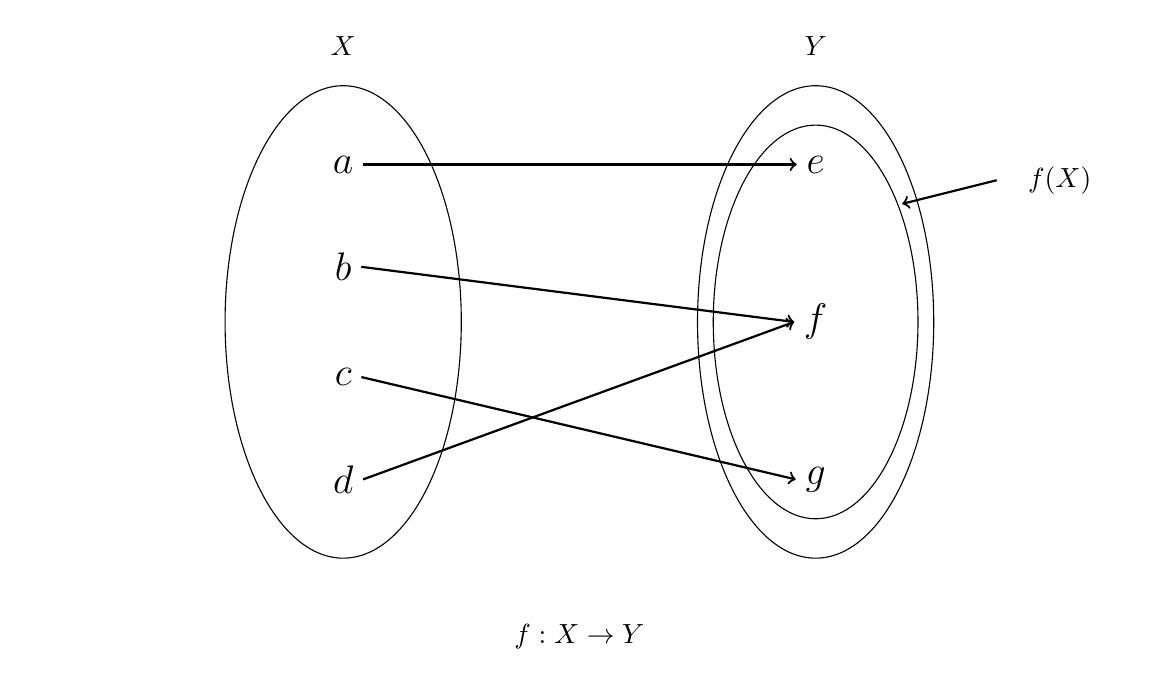
\begin{tikzpicture}
		\filldraw[white] (-7,-3) rectangle (7,3);
			
		\draw (-3,0) ellipse (1.5 and 3) node[yshift=3.5cm] {$X$};
		
		\draw (3,0) ellipse (1.5 and 3) node[yshift=3.5cm] {$Y$};
		\draw (3,0) ellipse (1.3 and 2.5);
		\draw[thick, ->] (5.3,1.8) node[xshift=.8cm] {$f(X)$} -- (4.1,1.5);
		
		\node (a) at (-3,2) {\Large$a$};
		\node (b) at (-3,.7) {\Large$b$};
		\node (c) at (-3,-.7) {\Large$c$};
		\node (d) at (-3,-2) {\Large$d$};
		
		\node (e) at (3,2) {\Large$e$};
		\node (f) at (3,0) {\Large$f$};
		\node (g) at (3,-2) {\Large$g$};
		
		\draw[thick,->] (a.east) -- (e.west);
		\draw[thick,->] (b.east) -- (f.west);
		\draw[thick,->] (c.east) -- (g.west);
		\draw[thick,->] (d.east) -- (f.west);
		
		\draw (0,-4) node {$f:X\to Y$};

	\end{tikzpicture}}
	\caption{}
	\label{fig:sur}
\end{figure}

\begin{figure}[h]
\centering
\resizebox{0.7\linewidth}{!}{
	\begin{tikzpicture}
		\filldraw[white] (-7,-3) rectangle (7,3);
			
		\draw (-3,0) ellipse (1.5 and 3) node[yshift=3.5cm] {$X$};
		
		\draw (3,0) ellipse (1.5 and 3) node[yshift=3.5cm] {$Y$};
		\draw (3,0) ellipse (1.3 and 2.5);
		\draw[thick, ->] (5.3,1.8) node[xshift=.8cm] {$f(X)$} -- (4.1,1.5);
		
		\node (a) at (-3,2) {\Large$a$};
		\node (b) at (-3,0) {\Large$b$};
		\node (c) at (-3,-2) {\Large$c$};
		
		\node (d) at (3,2) {\Large$d$};
		\node (e) at (3,0) {\Large$e$};
		\node (f) at (3,-2) {\Large$f$};
		
		\draw[thick,->] (a.east) -- (e.west);
		\draw[thick,->] (b.east) -- (f.west);
		\draw[thick,->] (c.east) -- (d.west);
		
		\draw (0,-4) node {$f:X\to Y$};

	\end{tikzpicture}}
	\caption{}
	\label{fig:bi}
\end{figure}

Before we talk about inverses, we must talk about functional composition. When we compose functions, all we are doing is taking the output from one function and putting it into another function. Because of some of the properties of this operation, the symbol we use for this looks very similar to multiplication.\footnote{If you ever take linear algebra, functional composition distributes on addition very similarly to how multiplication does. It also has an interesting connection to matrix multiplication, which is where I assume we get the symbol from (I'm not one hundred percent sure).}

\begin{figure}[h]
\centering
\resizebox{0.8\linewidth}{!}{
	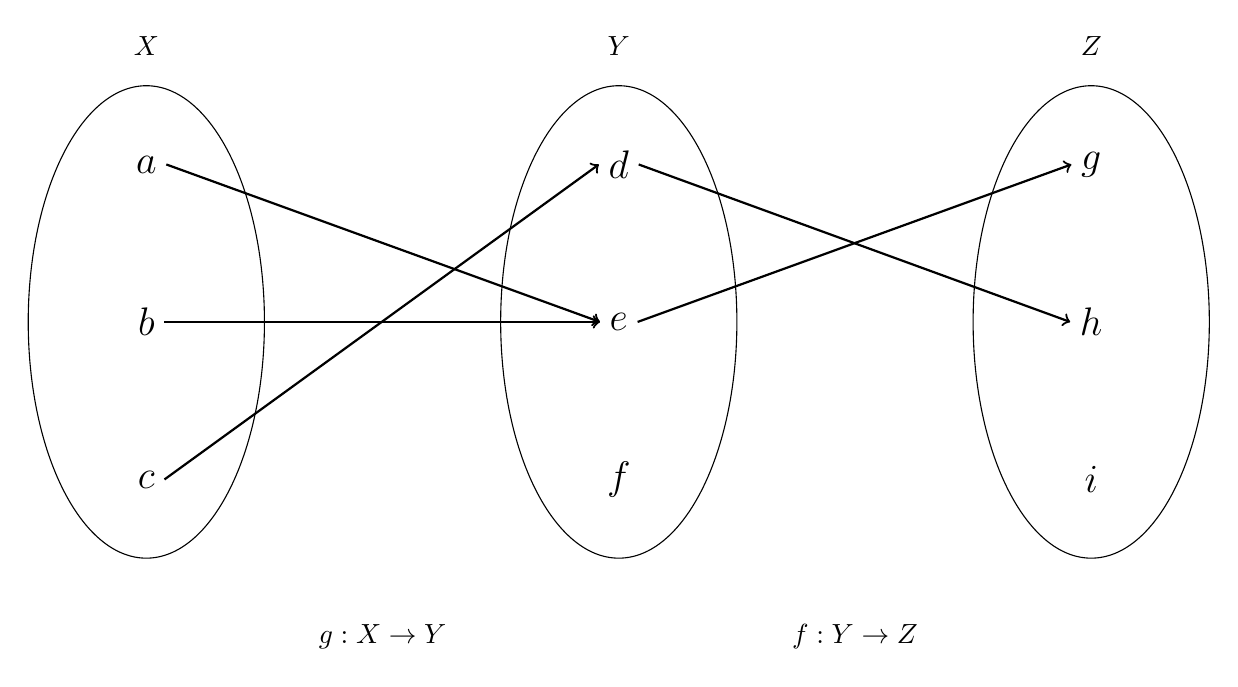
\begin{tikzpicture}
		\draw (-3,0) ellipse (1.5 and 3) node[yshift=3.5cm] {$X$};
		
		\draw (3,0) ellipse (1.5 and 3) node[yshift=3.5cm] {$Y$};
		
		\draw (9,0) ellipse (1.5 and 3) node[yshift=3.5cm] {$Z$};
				
		\node (a) at (-3,2) {\Large$a$};
		\node (b) at (-3,0) {\Large$b$};
		\node (c) at (-3,-2) {\Large$c$};
		
		\node (d) at (3,2) {\Large$d$};
		\node (e) at (3,0) {\Large$e$};
		\node (f) at (3,-2) {\Large$f$};
		
		\node (g) at (9,2) {\Large$g$};
		\node (h) at (9,0) {\Large$h$};
		\node (i) at (9,-2) {\Large$i$};
		
		\draw[thick,->] (a.east) -- (e.west);
		\draw[thick,->] (b.east) -- (e.west);
		\draw[thick,->] (c.east) -- (d.west);
		
		\draw[thick,->] (e.east) -- (g.west);
		\draw[thick,->] (d.east) -- (h.west);
		
		\draw (0,-4) node {$g:X\to Y$};
		\draw (6,-4) node {$f:Y\to Z$};
	\end{tikzpicture}}
	\caption{}
	\label{fig:comp}
\end{figure}

\begin{define}
	Define $f:Y\to Z$ and $g:X\to Y$. The composition of $f$ and $g$, notated as $f\circ g$ is a function $f\circ g:X\to Z$ such that $(f\circ g)(x)=f(g(x))$, or as seen in figure \eqref{fig:comp}.
\end{define}

An important property that's useful lmater, is that functional composition is associative, or $f\circ (g\circ h)=(f\circ g) \circ h$. The proof is trivial, so we ignore it here.

\begin{define}
\label{def:left}
	Define $f:X\to Y$. If there exists $g:Y\to X$ such that $g\circ f=I_X$, then $g$ is said to be the left inverse (retraction) of $f$.
	\end{define}
$I_X$ in definition \eqref{def:left} is simpily the identity function on domain $X$, where $I_X(x)=x$. Like how the symbol 1 works with multiplication, any composition with the identity function results in the same function (e.g. $f\circ I=I\circ f=f$).
\begin{define}
	Define $f:X\to Y$. If there exists $g:Y\to X$ such that $f\circ g=I_Y$, then $g$ is said to be the right inverse (section) of $f$. 
\end{define}

The left inverse is illustrated by figure \eqref{fig:left}.
\begin{figure}[h]
\centering
\resizebox{0.8\linewidth}{!}{
	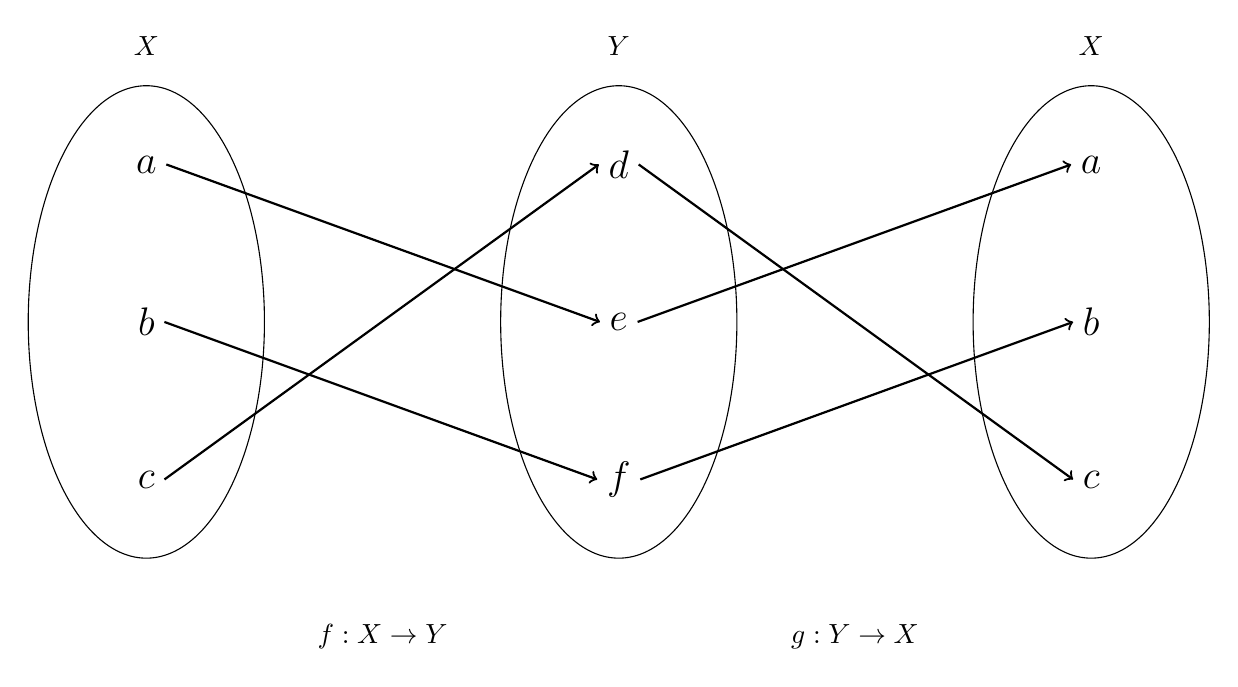
\begin{tikzpicture}
		\draw (-3,0) ellipse (1.5 and 3) node[yshift=3.5cm] {$X$};
		
		\draw (3,0) ellipse (1.5 and 3) node[yshift=3.5cm] {$Y$};
		
		\draw (9,0) ellipse (1.5 and 3) node[yshift=3.5cm] {$X$};
				
		\node (a) at (-3,2) {\Large$a$};
		\node (b) at (-3,0) {\Large$b$};
		\node (c) at (-3,-2) {\Large$c$};
		
		\node (d) at (3,2) {\Large$d$};
		\node (e) at (3,0) {\Large$e$};
		\node (f) at (3,-2) {\Large$f$};
		
		\node (g) at (9,2) {\Large$a$};
		\node (h) at (9,0) {\Large$b$};
		\node (i) at (9,-2) {\Large$c$};
		
		\draw[thick,->] (a.east) -- (e.west);
		\draw[thick,->] (b.east) -- (f.west);
		\draw[thick,->] (c.east) -- (d.west);
		
		\draw[thick,->] (e.east) -- (g.west);
		\draw[thick,->] (f.east) -- (h.west);
		\draw[thick,->] (d.east) -- (i.west);
		
		\draw (0,-4) node {$f:X\to Y$};
		\draw (6,-4) node {$g:Y\to X$};
	\end{tikzpicture}}
	\caption{}
	\label{fig:left}
\end{figure}
As you can see, a left inverse, essentially \textit{retracts} everything that $f$ has done and sends everyone back to where they came from.
The right inverse, as seen in figure \eqref{fig:right}
\begin{figure}[h]
\centering
\resizebox{0.8\linewidth}{!}{
	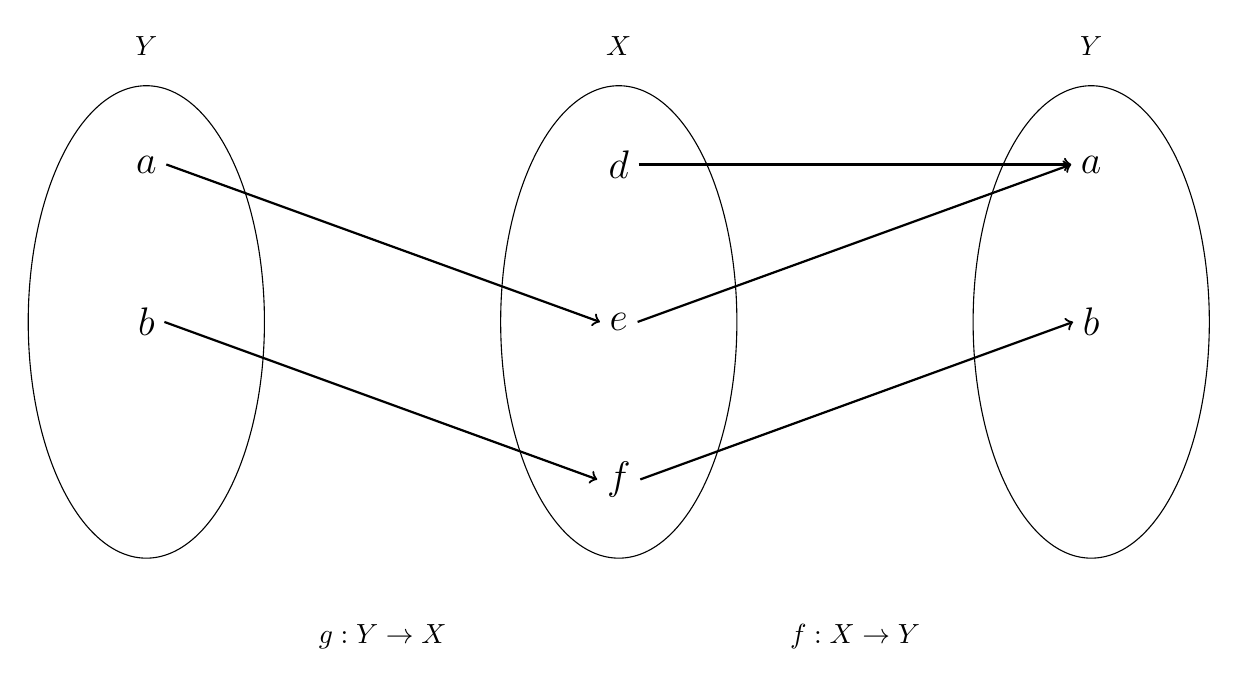
\begin{tikzpicture}
		\draw (-3,0) ellipse (1.5 and 3) node[yshift=3.5cm] {$Y$};
		
		\draw (3,0) ellipse (1.5 and 3) node[yshift=3.5cm] {$X$};
		
		\draw (9,0) ellipse (1.5 and 3) node[yshift=3.5cm] {$Y$};
				
		\node (a) at (-3,2) {\Large$a$};
		\node (b) at (-3,0) {\Large$b$};
		
		\node (d) at (3,2) {\Large$d$};
		\node (e) at (3,0) {\Large$e$};
		\node (f) at (3,-2) {\Large$f$};
		
		\node (g) at (9,2) {\Large$a$};
		\node (h) at (9,0) {\Large$b$};
		
		\draw[thick,->] (a.east) -- (e.west);
		\draw[thick,->] (b.east) -- (f.west);

		
		\draw[thick,->] (e.east) -- (g.west);
		\draw[thick,->] (f.east) -- (h.west);
		\draw[thick,->] (d.east) -- (g.west);
		
		\draw (0,-4) node {$g:Y\to X$};
		\draw (6,-4) node {$f:X\to Y$};
	\end{tikzpicture}}
	\caption{}
	\label{fig:right}
\end{figure}
is a function that takes a \textit{section} of the domain of $f$ and reverses it.

\begin{theorem}
\label{thm:left}
Define $f:X\to Y$. If $f$ has a left inverse, then $f$ is one-to-one.	
\end{theorem}
\begin{proof}
	Suppose $f$ is not one-to-one. Then there exists $x_1,x_2\in X$, $x_1\neq x_2$ such that $f(x_1)=f(x_2)$. Then let $g:Y\to X$ be the left inverse of $f$. Therefore
	$$g(f(x_1))=g(f(x_2))$$
	by $f(x_1)=f(x_2)$ and the defintion of a function.
	But since $g\circ f=I_x$, we deduce
	$$x_1=x_2$$
	which is a contradiction, hence proving $f$ is one-to-one.
\end{proof}

\begin{theorem}
\label{thm:right}
Define $f:X\to Y$. If $f$ has a right inverse, then $f$ is a surjection.
\end{theorem}
\begin{proof}
Exercise.	
\end{proof}

\begin{define}
	Define $f:X\to Y$. If $f$ has left inverse $g:Y\to X$ and right inverse $h:y\to X$, then $f$ is said to have a two-sided inverse.
	$$f^{-1}=g=h$$
\end{define}
From here on out, I will use the term inverse, for a two-sided inverse.
\begin{theorem}
\label{thm:bi}
Suppose $f:X\to Y$ has an inverse, then $f$ is a bijection.
\end{theorem}
\begin{proof}
	By theorems \eqref{thm:left} and \eqref{thm:right}, $f$ is both one-to-one and onto, concluding that $f$ is a bijection.
\end{proof}

Now from theorem \eqref{thm:bi} inverses can only be constructed for bijective functions. 
While this might be true by the strict definition of an inverse, there are ways in which we can build meaningful inverses by changing the function definition just a little bit. 
An example of this would be the inverse trig functions. Just by inspection of the plots of any trig function, an immediate conclusion is that they are not one-to-one. But somehow, the inverses for these functions are still defined. In this next section, we will explore how this is possible.

\begin{lemma}
\label{lem:in-to-bi}
Let $f:X\to Y$ be one-to-one. Then there exists a bijection $g:X\to Z$, where for any $x\in X$, $f(x)=g(x)$.
\end{lemma}
\begin{proof}
To prove our theorem, let's define $Z=f(X)$. Then as defined in the theorem, we need to prove $g$ is a bijection. Trivially, $g$ is one-to-one since $f$ is one-to-one. Then by the definition of the image, every $z\in Z$ has a corresponding $x\in X$ hence proving $g$ is a bijection.
\end{proof}
\begin{theorem}
\label{thm:to-bi}
Let $f:X\to Y$ be any arbitrary function. Then there exists a bijection $g:A\to B$ such that $A\subseteq X$, $B\subseteq B$, and for any $a\in A$,
$$f(a)=g(a)$$
\end{theorem}
\begin{proof}
	To prove this theorem, we first establish the existence of an intermediate function, ${h:A\to Y}$ that is one-to-one. Let every element $x\in A$ such that for $y=f(x)$, $y$ only has one corresponding input be in $A$. Then for the elements $x\in X$ such that for $y=f(x)$ has multiple corresponding inputs, we chose just one to be in $A$.\footnote{We can do this because of the Axiom of Choice if we choose to believe in its validity.}
	Therefore, by the definition of $A$, $h$ must be one-to-one. Then by lemma \eqref{lem:in-to-bi}, we can construct $g:A\to B$ which is bijective, hence completing the proof. 
\end{proof}

Now with theorem \eqref{thm:to-bi}, we now know we can transform any function into a bijection, which has an inverse. With this, let's try this in an example.
\begin{ex}
	Let's try to construct a meaningful inverse for the function
	$$f(x)=\sqrt{x},$$
	where $f:[0,\infty)\to \real$.
	By imagining the function's plot in our heads, $f$ is one-to-one but isn't onto. Since we know $f$ doesn't output anything less than 0, we can construct a new function 
	$$g(x)=f(x)$$
	where $g:[0,\infty)\to [0,\infty)$. Now checking, $g$ is clearly onto, since the image is exactly equal to the codomain, our new function $g$ is a bijection, therefore there exists $g^{-1}$ such that
	$$g^{-1}\circ g=g\circ g^{-1}=I_{[0,\infty)}$$
	Doing some simple algebra, we get
	$$g^{-1}(x)=x^2.\footnotemark$$
	\footnotetext{Even though it's trivial, check this is indeed the case by computing $g^{-1}\circ g$ and $g\circ g^{-1}$.}
\end{ex}

\begin{ex}
	In this next example let's try to determine the domain and codomain of $\sin^{-1}(x)$. By imagining the plot of $f(x)=\sin(x)$, we conclude that $f$ is not one-to-one nor onto. We first solve the onto problem by setting our new function's codomain to $f(X)$, which in this case is $[-1,1]$. 
	Like in the proof of theorem \eqref{thm:to-bi}, there is a choice involved here, so unlike in the previous example, answers can vary depending on what we'd like to achieve. For our purposes, we will cut the number line leaving the interval $(-\frac{\pi}{2},\frac{\pi}{2}]$. We can check this is the case by plotting $f$ on the domain, and $f$ passes the horizontal line test. Hence we define $g: (-\frac{\pi}{2},\frac{\pi}{2}] \to [-1,1]$, where
	$$g(x)=\sin(x)$$
	and
	$$g^{-1}=\sin^{-1}(x)$$
	where $g^{-1}: [-1,1] \to (-\frac{\pi}{2},\frac{\pi}{2}]$.
\end{ex}

\begin{ex}
	In this example, we'd like to find a meaningful inverse for
	$$f(x)=\frac{x}{1+x}$$
	for the largest possible domain $X$, where $X\subseteq \real$. We conclude our largest possible domain is $X=\{x\in\real : x\neq -1\}$. Then we wish to define the codomain of $f$ such that $f$ is onto. We have not learned how to compute this at the moment, so I will state without proof that $1$ is not related to any element in the domain. Therefore, we can let 
	$$f:\real \setminus \{-1\} \to \real \setminus \{1\}.$$
	Then to find the graph of $f$, we will solve this algebraically. Let $y=f(x)$ for any $x$. Then
	$$y=\frac{x}{1+x}$$
	which by eliminating the dominator, we get
	$$y+xy=x$$
	hence
	$$y=x-xy$$
	$$y=x(1-y)$$
	$$x=\frac{y}{1-y}$$
	Then letting $f^{-1}(y)=x$, we get the graph of $f^{-1}$ is
	$$f^{-1}(x)=\frac{x}{1-x}\footnotemark$$
	\footnotetext{I just switch $x$ and $y$, for if anyone is confused. It just looks better this way. If you'd like, just substitute in $y$ to get $f^{-1}(y)$.}
	We can check that this is indeed the inverse by computing
	$$f(f^{-1}(x))=\frac{f^{-1}(x)}{1+f^{-1}(x)}=\frac{\frac{x}{1-x}}{1+\frac{x}{1-x}}$$
	$$=\frac{x}{(1-x)+x}=x=I$$
	and
	$$f^{-1}(f(x))=\frac{f(x)}{1-f(x)}=\frac{\frac{x}{1+x}}{1-\frac{x}{1+x}}$$
	$$=\frac{x}{(1+x)-x}=x=I\footnotemark$$
	\footnotetext{If you notice, finding the max domain for $f^{-1}$, we get the set $\real\setminus\{1\}$ which is exactly the image of $f$. 
	I mentioned that computing the image for $f$ might be tricky, but another way we can look at it is if we compute the graph of $f$, we can use the domain of the graph, which is usually easier to compute to compute the image of $f$. 
	This is of course relying on the fact the inverse is possible to compute algebraically since some are not possible given our tools of algebra.}
\end{ex}

\section{Exercises}
\end{document}









